%%%%%%%%%%%%%%%%%%%%%%%%%%%%%%%%%%%%%%%%%
% Beamer Presentation
% LaTeX Template
% Version 1.0 (10/11/12)
%
% This template has been downloaded from:
% http://www.LaTeXTemplates.com
%
% License:
% CC BY-NC-SA 3.0 (http://creativecommons.org/licenses/by-nc-sa/3.0/)
%
%%%%%%%%%%%%%%%%%%%%%%%%%%%%%%%%%%%%%%%%%

%----------------------------------------------------------------------------------------
%	PACKAGES AND THEMES
%----------------------------------------------------------------------------------------

\documentclass[xcolor=svgnames]{beamer}

\mode<presentation> {

% The Beamer class comes with a number of default slide themes
% which change the colors and layouts of slides. Below this is a list
% of all the themes, uncomment each in turn to see what they look like.

% \usetheme{default}
% \usetheme{AnnArbor}
% \usetheme{Antibes}
%\usetheme{Bergen}
% \usetheme{Berkeley}
% \usetheme{Berlin}
\usetheme{Boadilla}
% \usetheme{CambridgeUS}
% \usetheme{Copenhagen}
% \usetheme{Darmstadt}
% \usetheme{Dresden}
% \usetheme{Frankfurt}
% \usetheme{Goettingen}
% \usetheme{Hannover}
% \usetheme{Ilmenau}
% \usetheme{JuanLesPins}
% \usetheme{Luebeck}
% \usetheme{Madrid}
% \usetheme{Malmoe}
% \usetheme{Marburg}
% \usetheme{Montpellier}
% \usetheme{PaloAlto}
% \usetheme{Pittsburgh}
% \usetheme{Rochester}
% \usetheme{Singapore}
% \usetheme{Szeged}
% \usetheme{Warsaw}

% As well as themes, the Beamer class has a number of color themes
% for any slide theme. Uncomment each of these in turn to see how it
% changes the colors of your current slide theme.

% \usecolortheme{albatross}
% \usecolortheme{beaver}
%\usecolortheme{beetle}
% \usecolortheme{crane}
%  \usecolortheme{dolphin}
% \usecolortheme{dove}
% \usecolortheme{fly}
% \usecolortheme{lily}
% \usecolortheme{orchid}
% \usecolortheme{rose}
% \usecolortheme{seagull}
% \usecolortheme{seahorse}
% \usecolortheme{whale}
% \usecolortheme{wolverine}

% \setbeamertemplate{footline} % To remove the footer line in all slides uncomment this line
%\setbeamertemplate{footline}[page number] % To replace the footer line in all slides with a simple slide count uncomment this line

% \setbeamertemplate{navigation symbols}{} % To remove the navigation symbols from the bottom of all slides uncomment this line
}

\usepackage{graphicx} % Allows including images
\usepackage{booktabs} % Allows the use of \toprule, \midrule and \bottomrule in tables
\usepackage{tikz}
\usepackage{multicol}
\usepackage{wrapfig}
\usepackage{amsmath,amsthm,amssymb}
\usepackage{mathtools}
\usepackage{hyperref}
\DeclarePairedDelimiter\ceil{\lceil}{\rceil}
\DeclarePairedDelimiter\floor{\lfloor}{\rfloor}


\addtobeamertemplate{frametitle}{}{%
\begin{tikzpicture}[remember picture,overlay]
\node[anchor=north east,yshift=2pt] at (current page.north east) {
\includegraphics[height=0.8cm]{iiit-new.png}};
\end{tikzpicture}}

\setbeamercolor{title in head/foot}{bg=OrangeRed, fg=White}
\setbeamercolor{author in head/foot}{bg=RoyalBlue, fg=White}
\setbeamercolor{date in head/foot}{bg=SlateGray, fg=Black}

%----------------------------------------------------------------------------------------
%	TITLE PAGE
%----------------------------------------------------------------------------------------

\title[Discrete Structures]{Discrete Structures} % The short title appears at the bottom of every slide, the full title is only on the title page
\author{IIIT Hyderabad} % Your name
\institute[] % Your institution as it will appear on the bottom of every slide, may be shorthand to save space
{
Monsoon 2020 \\ % Your institution for the title page
\medskip
\textit{Tutorial 6} % Your email address
}
\date{October 5, 2020} % Date, can be changed to a custom date

\begin{document}

\begin{frame}
\titlepage % Print the title page as the first slide
\end{frame}

\begin{frame}
\frametitle{Introduction} % Table of contents slide, comment this block out to remove it
\tableofcontents % Throughout your presentation, if you choose to use \section{} and \subsection{} commands, these will automatically be printed on this slide as an overview of your presentation
\end{frame}

%----------------------------------------------------------------------------------------
%	PRESENTATION SLIDES
%----------------------------------------------------------------------------------------
\section{This Tutorial}
\begin{frame}{This Tutorial}
    \begin{itemize}
        \item Solving till 1:30PM. After that 2 separate meets.
        \item After that, doubts till now, about any topic covered.
        \item Please join the meets as per roll number - 
        \begin{enumerate}
            \item Roll Number 2020909122-37 : Vikrant
            \item Roll Number 2020909138-54 : Jai
        \end{enumerate}
    \end{itemize}
\end{frame}


%------------------------------------------------
\section{Questions}
%------------------------------------------------

%------------------------------------------------
\subsection{Question 1}
%------------------------------------------------
\begin{frame}{Question 1}
    Consider elliptic curve $E_{5}(2,1)$ or in equation form as -
    \begin{align*}
        y^2 &= x^3 + 2x + 1
    \end{align*}
    \textbf{1.1:}: Find all points in the curve.
    \\ \textbf{\underline{Sol:}} Use the following algorithm - 
    \begin{center}
        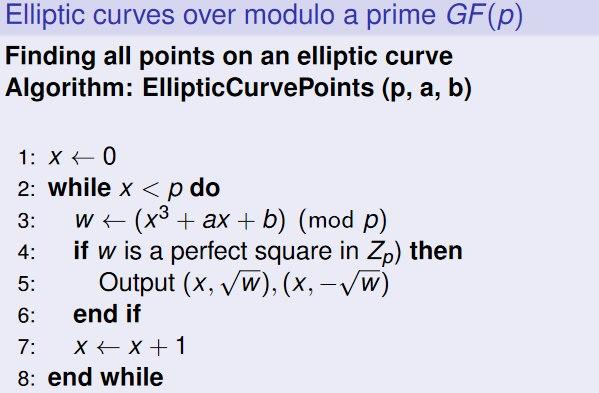
\includegraphics[width=0.5\linewidth]{photo_2020-10-04_14-12-31.jpg}
    \end{center}
\end{frame}
\begin{frame}{}
    \begin{enumerate}
        \item x = 0, w = 1, output (0,1) and  (0,-1 )or (0,4). 
        \item x = 1, w = 4, output (1,2) and (1,-2) or (1,3).
        \item x = 2, w = 13 = 3, not perfect square. 
        \item x = 3, w = 34 = 4, output (3,3) and (3,-3) or (3,2).
        \item x = 4, w = 3, not perfect square.
    \end{enumerate}
    Thus we get (0,1),(0,4),(1,2),(1,3),(3,3) and (3,1).
    \vspace{1cm}
    \\ \textbf{1.2:} If $P=(1,3)$ and $Q = (3,2)$ lie on the above curve, find - 
    \begin{enumerate}
        \item -P
        \\ \textbf{\underline{Sol:}} It would be (1,-3) or (1,2). As $3 + 2 = 5$.
    \end{enumerate}    
\end{frame}
\begin{frame}
    \begin{enumerate}\setcounter{enumi}{1}
        \footnotesize{
        \item P + Q
        \\ \textbf{\underline{Sol:}} We need to compute $R = P+Q$. 
        \begin{align*}
            \lambda &= \frac{2 - 3}{3 - 1} = \frac{-1}{2}
                \\   &= \frac{4}{2} = 2
                \\ x_R &= 4 - x_P - x_Q
                \\ &= 0
                \\ y_R &= 2(x_P - x_R) - y_P
                \\ &= -1 = 4
        \end{align*}
        Thus we get (0,4).
        \item 2Q
        \begin{align*}
            \lambda &= \frac{3\cdot 9 + 2}{4}
                \\  &= 1
                \\ x_R &= 1 - x_Q - x_Q
                \\ &= -5 = 0
                \\ y_R &= 1(x_Q - x_R) - y_Q
                \\ &= 1
        \end{align*}
        Thus we get (0,1).    
        }
        
    \end{enumerate}
\end{frame}
\end{document} 